% https://tex.stackexchange.com/questions/394815/can-i-represent-the-beam-deflection-curve-with-the-stanli-package
\documentclass{scrartcl}
\usepackage{stanli}
\usetikzlibrary{decorations.pathreplacing}

\begin{document}
  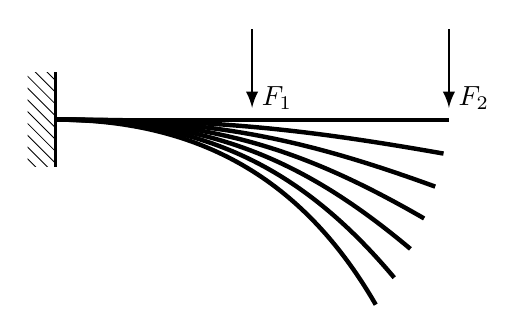
\begin{tikzpicture}
    %the points
    \point{begin}{0}{0};
    \point{middle}{2.5}{0};
    \point{end}{5}{0};
    %the beam
    \beam{2}{begin}{end};
    %the support
    \support{3}{begin}[-90];
    %the load
    \load{1}{middle}[90];
    \load{1}{end}[90];
    %the inscription of the load
    \notation{1}{middle}{$F_1$};
    \notation{1}{end}{$F_2$};
    %the deflection curves
% without correction
%    \foreach [evaluate={\in=180-\b*2}] \b in {5,10,...,30}
%      \draw[red,-, ultra thick] (begin) to[out=0,in=\in] (-\b:5);
% quater circle with full radius
%    \draw[red] (begin) -- (end) arc (0:-90:5) -- cycle;
% polar coordinates with some correction of the radius to account for bend
    \foreach [evaluate={\in=180-\b*2}] \b in {5,10,...,30}{
      \draw[-, ultra thick] (begin) to[out=0,in=\in] (-\b:5-\b*0.01);
% quater circles with sortened radius
%      \draw[red] (begin) -- (5-\b*0.01,0) arc (0:-90:5-\b*0.01) -- cycle;
    }
  \end{tikzpicture}
\end{document}

%%% Local Variables:
%%% mode: latex
%%% TeX-master: t
%%% End:
